\documentclass[border=4pt,12pt]{standalone}
% House style for redrawn exam diagrams (diagram-v4: 0.4pt lines, filled -latex arrows, fine dashes; stipple and hatching drawn as real dots/lines (no PDF/SVG patterns, so they render in every browser and at any scale); transparent background). Every figure \input's this.
\usepackage{amsmath,amssymb}
\usepackage{txfonts}
\usepackage{pdfrender,xcolor}
% \halo{text}: label on shading. The shading stops just around each letter's outline (a thin knock-out that follows the
% glyphs, like the papers' typesetting), never a box. Owner: "I don't want a box around the text".
\newcommand{\halo}[1]{\leavevmode\rlap{\pdfrender{TextRenderingMode=2,LineWidth=2.2pt,LineJoinStyle=1,StrokeColor=white,FillColor=white}#1}#1}
\usepackage{tikz,pgfplots}
\pgfplotsset{compat=1.18}
\usetikzlibrary{arrows.meta,calc,angles,quotes,patterns,patterns.meta,intersections,positioning,decorations.markings,shapes.geometric}
% Stipple and hatching are drawn as actual dots / lines clipped to the region (path picture), NOT as pattern fills:
% SVG <pattern> fills vanish or blur when browsers scale the image, so the owner could not see the shading.
% Each dot is a 0.72pt square (keeps SVGs small; reads as a dot at print size). Dots sit on one global staggered grid, so neighbouring regions line up.
\makeatletter
\newdimen\ex@x \newdimen\ex@y \newdimen\ex@xa \newdimen\ex@ya \newdimen\ex@xb \newdimen\ex@yb \newcount\ex@row
\def\exam@stipplecolor{black!75}\def\exam@dotr{0.42pt}\def\exam@dotgap{2.5}
\def\ex@rowdots{\ifdim\ex@x<\ex@xb \pgfpathrectangle{\pgfqpoint{\dimexpr\ex@x-0.36pt\relax}{\dimexpr\ex@y-0.36pt\relax}}{\pgfqpoint{0.72pt}{0.72pt}}\advance\ex@x by \exam@dotgap pt\relax\expandafter\ex@rowdots\fi}
\def\exam@stipple{%
  \pgftransformreset% dots are sized in real points even inside scaled pictures
  \pgfpointanchor{path picture bounding box}{south west}\ex@xa=\pgf@x \ex@ya=\pgf@y
  \pgfpointanchor{path picture bounding box}{north east}\ex@xb=\pgf@x \ex@yb=\pgf@y
  \pgfsetfillcolor{\exam@stipplecolor}\pgfmathsetmacro\ex@h{\exam@dotgap/2}%
  \pgfmathtruncatemacro\ex@r{floor(\ex@ya/\ex@h)-1}\ex@row=\ex@r\relax
  \ex@y=\ex@r\dimexpr\ex@h pt\relax
  \loop\ifdim\ex@y<\ex@yb
    \pgfmathtruncatemacro\ex@c{floor(\ex@xa/\exam@dotgap)-1}\ex@x=\ex@c\dimexpr\exam@dotgap pt\relax
    \ifodd\ex@row \advance\ex@x by \ex@h pt\fi
    \ex@rowdots
    \advance\ex@y by \ex@h pt \advance\ex@row by 1
    \ifnum\numexpr\ex@row-(\ex@row/4)*4\relax=0 \pgfusepath{fill}\fi% flush every 4 rows: bounded TeX memory, few clip copies in the SVG
  \repeat\pgfusepath{fill}}
\newdimen\ex@d
\def\exam@hatch#1{% #1 = 1 for /, -1 for \ ; lines 45 degrees, 3pt apart
  \pgftransformreset
  \pgfpointanchor{path picture bounding box}{south west}\ex@xa=\pgf@x \ex@ya=\pgf@y
  \pgfpointanchor{path picture bounding box}{north east}\ex@xb=\pgf@x \ex@yb=\pgf@y
  \ex@d=\dimexpr\ex@yb-\ex@ya\relax \ex@x=\dimexpr\ex@xa-\ex@d\relax
  \loop\ifdim\ex@x<\ex@xb
    \ifnum#1>0 \pgfpathmoveto{\pgfqpoint{\ex@x}{\ex@ya}}\pgfpathlineto{\pgfqpoint{\dimexpr\ex@x+\ex@d\relax}{\ex@yb}}%
    \else \pgfpathmoveto{\pgfqpoint{\ex@x}{\ex@yb}}\pgfpathlineto{\pgfqpoint{\dimexpr\ex@x+\ex@d\relax}{\ex@ya}}\fi
    \advance\ex@x by 4.24pt
  \repeat
  \pgfsetlinewidth{0.4pt}\pgfsetstrokecolor{black}\pgfusepath{stroke}}
\def\examstipple{\exam@stipple}\def\examhatch{\exam@hatch}\def\examsetstipplecolor#1{\def\exam@stipplecolor{#1}}\def\examsetdotgap#1{\def\exam@dotgap{#1}}
\makeatother
% (legacy pattern kept for old files)
% staggered stipple like the NESA papers' dotted shading
\pgfdeclarepatternformonly{exam stipple}{\pgfpointorigin}{\pgfqpoint{2.2pt}{2.2pt}}{\pgfqpoint{2.2pt}{2.2pt}}{%
  \pgfpathcircle{\pgfqpoint{0.55pt}{0.55pt}}{0.42pt}\pgfpathcircle{\pgfqpoint{1.65pt}{1.65pt}}{0.42pt}\pgfusepath{fill}}
\tikzset{
  every picture/.style={line width=0.6pt, >={Latex[length=2mm,width=1.3mm]}},
  curve/.style={line width=0.6pt},
  open arrow/.style={-{Latex[length=2mm,width=1.3mm]}},  % owner: filled -latex heads everywhere, no open chevrons
  aux/.style={dash pattern=on 2pt off 1.5pt, line width=0.6pt},
  shade/.code={\def\exA{#1}\def\exB{none}\ifx\exA\exB\else\pgfkeysalso{fill=black!18}\fi},
  shade/.default=on,
  shade dots/.style={fill=none, path picture={\examstipple}},
  stipple color/.code={\examsetstipplecolor{#1}},
  stipple gap/.code={\examsetdotgap{#1}},
  shade dense dots/.style={fill=none, stipple gap=1.6, path picture={\examstipple}},
  shade hatch/.style={fill=none, path picture={\examhatch{1}}},
  shade hatch reverse/.style={fill=none, path picture={\examhatch{-1}}},
  shade solid/.style={fill=black},
  pt/.style={circle, fill, inner sep=1.1pt},
  open pt/.style={circle, draw, fill=white, inner sep=1.1pt},
}
\pgfplotsset{
  exam axes/.style={axis lines=middle, axis line style={->}, xlabel={$x$}, ylabel={$y$},
    xlabel style={anchor=west}, ylabel style={anchor=south}, tick label style={font=\small},
    every axis plot/.append style={line width=0.6pt, black}, samples=200, clip=false,
    enlargelimits=false, axis on top},
}

\begin{document}
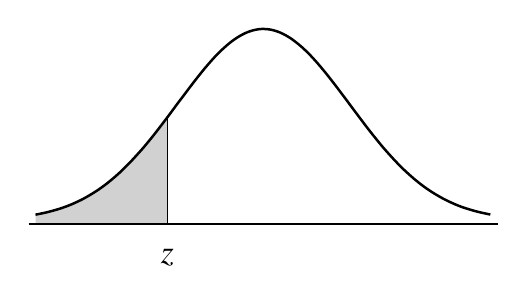
\begin{tikzpicture}[x=0.0127cm,y=-0.0127cm,font=\fontsize{12}{14.399999999999999}\selectfont]
\fill[shade] (35,214.5)--plot[smooth] coordinates {(35.0,205.4) (38.4,204.8) (41.8,204.1) (45.2,203.3) (48.5,202.5) (51.9,201.6) (55.3,200.6) (58.7,199.6) (62.1,198.5) (65.5,197.3) (68.8,196.0) (72.2,194.6) (75.6,193.1) (79.0,191.5) (82.4,189.7) (85.8,187.9) (89.2,186.0) (92.5,183.9) (95.9,181.8) (99.3,179.5) (102.7,177.0) (106.1,174.5) (109.5,171.8) (112.8,169.0) (116.2,166.0) (119.6,162.9) (123.0,159.7) (126.4,156.4) (129.8,152.9) (133.2,149.3) (136.5,145.6) (139.9,141.8) (143.3,137.9) (146.7,133.8) (150.1,129.7) (153.5,125.5) (156.8,121.2) (160.2,116.8) (163.6,112.4) (167.0,107.9)}--(167,214.5)--cycle;
\draw (28,214.5)--(498,214.5);
\draw[line width=0.9pt] plot[smooth] coordinates {(35.0,205.4) (40.1,204.4) (45.2,203.3) (50.3,202.0) (55.4,200.6) (60.6,199.0) (65.7,197.2) (70.8,195.2) (75.9,192.9) (81.0,190.5) (86.1,187.7) (91.2,184.7) (96.3,181.5) (101.5,177.9) (106.6,174.1) (111.7,169.9) (116.8,165.5) (121.9,160.8) (127.0,155.7) (132.1,150.4) (137.2,144.8) (142.4,139.0) (147.5,132.9) (152.6,126.6) (157.7,120.1) (162.8,113.4) (167.9,106.7) (173.0,99.8) (178.1,92.9) (183.3,86.1) (188.4,79.3) (193.5,72.6) (198.6,66.1) (203.7,59.8) (208.8,53.8) (213.9,48.1) (219.0,42.8) (224.2,38.0) (229.3,33.6) (234.4,29.8) (239.5,26.6) (244.6,23.9) (249.7,21.9) (254.8,20.5) (259.9,19.7) (265.1,19.7) (270.2,20.3) (275.3,21.6) (280.4,23.5) (285.5,26.1) (290.6,29.2) (295.7,33.0) (300.8,37.2) (306.0,42.0) (311.1,47.2) (316.2,52.8) (321.3,58.8) (326.4,65.0) (331.5,71.5) (336.6,78.1) (341.7,84.9) (346.9,91.8) (352.0,98.7) (357.1,105.5) (362.2,112.3) (367.3,119.0) (372.4,125.5) (377.5,131.8) (382.6,138.0) (387.8,143.9) (392.9,149.5) (398.0,154.9) (403.1,160.0) (408.2,164.7) (413.3,169.2) (418.4,173.4) (423.5,177.3) (428.7,180.9) (433.8,184.2) (438.9,187.2) (444.0,190.0) (449.1,192.5) (454.2,194.8) (459.3,196.9) (464.4,198.7) (469.6,200.3) (474.7,201.8) (479.8,203.1) (484.9,204.2) (490.0,205.3)};
\draw (167,107.9)--(167,214.5);
\node[anchor=base,inner sep=0] at (167,254) {$z$};\end{tikzpicture}
\end{document}
